\section*{Seminár 24}

\subsection*{Téma}
Kombinatorika I~-- úlohy na mriežke a šachovnici
\subsection*{Ciele}
Zoznámiť študentov s metódami, ktoré si budú vyžadovať rôznorodé úlohy využívajúce šachovnice alebo tabuľky.

\subsection*{Úlohy a riešenia}
\begin{tcolorbox}[breakable,notitle,boxrule=0pt,colback=light-gray,colframe=light-gray]\ul{24.1} [66-II-2]
Štvorcovú tabuľku $6\times 6$ zaplníme všetkými celými číslami od 1 do 36.

a) Uveďte príklad takého zaplnenia tabuľky, že súčet každých dvoch čísel v~rovnakom riadku či v~rovnakom stĺpci je väčší ako 11.

b) Dokážte, že pri ľubovoľnom zaplnení tabuľky sa v~niektorom riadku alebo stĺpci nájdu dve čísla, ktorých súčet neprevyšuje 12.

\end{tcolorbox}

\rieh  a) Aby sme dosiahli požadované rozmiestnenie čísel v~tabuľke, nesmú v~žiadnom riadku ani stĺpci spolu zostať dve z~čísel nanajvýš rovných šiestim. Preto jednu z~mnohých vyhovujúcich tabuliek zostavíme, keď čísla od 1 do 6 vpíšeme zhora nadol do políčok jednej uhlopriečky a ďalej budeme postupne zdola nahor brať rady políčok rovnobežných s~druhou uhlopriečkou a do voľných miest každej z~nich vpisovať zhora
nadol zvyšné čísla 7, 8 atď. až 36:
\begin{center}
\begin{tabular}{|c|c|c|c|c|c|}
\hline
1 & 35 & 33 & 29 & 25 & 19 \\
\hline
36 & 2 & 30 & 26 & 20 & 15 \\
\hline
34 & 31 & 3 & 21 & 16 &11 \\
\hline
32 & 27 & 22 & 4 & 12 & 9 \\
\hline
28 & 23 & 17 & 13 & 5 & 7 \\
\hline
24 & 18 & 14 & 10 & 8 & 6\\
\hline
\end{tabular}
\end{center}
Najmenšie súčty dvoch čísel z~jednotlivých riadkov (zhora nadol) sú
$$1 + 19, 2 + 15, 3 + 11, 4 + 9, 5 + 7, 6 + 8$$
a z~jednotlivých stĺpcov (zľava doprava)
$$1 + 24, 2 + 18, 3 + 14, 4 + 10, 5 + 8, 6 + 7.$$
Rýchlejší opis príkladu vyhovujúcej tabuľky a jeho jednoduchšiu kontrolu dostaneme, keď do tabuľky vpíšeme iba čísla od 1 do 12, ako vidíme nižšie. Rozmiestnenie čísel od 13 do 36 do prázdnych políčok už zrejme môže byť ľubovoľné -- dve najmenšie čísla v~každom riadku aj stĺpci sú totiž práve tie od 1 do 12.
\begin{center}
\begin{tabular}{|c|c|c|c|c|c|}
\hline
1 & 11 & & & & \\
\hline
12 & 2 & & & & \\
\hline
 & & 3 & 9 & & \\
\hline
 & & 10 & 4 & & \\
\hline
 & & & & 5 & 7\\
\hline
 & & & & 8 & 6 \\
\hline
\end{tabular}
\end{center}

b) Ak sú dve z~čísel od 1 do 6 v~rovnakom riadku alebo v~rovnakom stĺpci, ich súčet neprevýši dokonca ani číslo $6 + 5 = 11$. V~opačnom prípade sú čísla od 1 do 6 rozmiestnené vo všetkých riadkoch a všetkých stĺpcoch, takže číslo 7 je v~rovnakom riadku s~číslom $x$ a v~rovnakom stĺpci s~číslom $y$, pričom $x$ a $y$ sú dve rôzne čísla od 1 do 6. Potom menšie z~čísel $7 + x$ a $7 + y$ neprevýši menšie z~čísel $7 + 6$ a $7 + 5$, teda číslo 12. Tým je tvrdenie dokázané.\\
\\
\kom Úloha je relatívne jednoduchá a nevyžaduje žiadne špeciálne matematické vedomosti, len starostlivý logický úsudok. Študenti pravdepodobne vymyslia rôzne zaplnenia tabuľky a to môže byť výbornou príležitosťou nechať ich riešenia skontrolovať si medzi sebou navzájom. \\
\\
\begin{tcolorbox}[breakable,notitle,boxrule=0pt,colback=light-gray,colframe=light-gray]\ul{24.2} [62-I-1-N1]
Kobylka skáče po úsečke dĺžky 10\,cm a to skokmi o~1\,cm alebo o~2\,cm (vždy rovnakým smerom). Koľkými spôsobmi sa môže dostať z~jedného krajného bodu úsečky do druhého?

\end{tcolorbox}

\rieh Ak označíme $a_n$ počet spôsobov, koľkými sa môže kobylka dostať do bodu vzdialeného $n$ cm od začiatočného bodu úsečky, tak pre každé $n \geq 1$ platí $a_{n+2}= a_{n+1} + a_n$. Keďže $a_1 = 1$ a $a_2 = 2$, môžeme ďalšie počty $a_3, a_4,\ldots$ postupne počítať podľa vzorca z~predošlej vety, až dospejeme k~hodnote $a_{10} = 89$.

Pri inom postupe je možné rozdeliť všetky cesty podľa toho, koľko pri nich urobí kobylka skokov dĺžky dva (ich počet môže byť 0, 1, 2, 3, 4 alebo 5 a tým je tiež určený počet skokov dĺžky $1$: 10, 8, 6, 4, 2 alebo 0). Ku každému takému počtu potom určíme počet všetkých rôznych poradí jednotiek a dvojok (dávajúcich v~súčte 10). Dostaneme tak $1+9+28+ 35 + 15 + 1 = 89$ možných ciest.\\
\\
\kom Úloha opäť pravdepodobne nebude pre študentov neprekonateľnou výzvou. Bude však určite zaujímavé sledovať, ako sa študenti popasujú s hľadaním počtu spôsobov. Taktiež úloha slúži ako príprava na úlohu nasledujúcu a domácu prácu.\\
\\
\begin{tcolorbox}[breakable,notitle,boxrule=0pt,colback=light-gray,colframe=light-gray]\ul{24.3} [62-I-2-N2, upravené] Škriatok sa pohybuje v~tabuľke $10 \times 15$ skokmi o~jedno políčko nahor alebo o~jedno políčko doprava. Koľkými rôznymi cestami sa môže dostať z~ľavého dolného do pravého horného políčka?\

\end{tcolorbox}

\rieh Škriatok urobí 9 skokov nahor a 14 skokov doprava. Jeho cestu určíme, keď v~poradí všetkých 23 skokov vyberieme tých deväť, ktoré povedú nahor. Počet týchto výberov 9 prvkov z~daných 23 je rovný zlomku $\frac{23 \cdot 22 \cdots 16 \cdot 15}{9 \cdot 8 \cdots2\cdot 1}$, teda číslu $817 190$.\\
\\
\kom Ako sme už spomínali, táto úloha je tiež prípravou na domácu prácu. Je tiež vhodným miestom, kde môžeme prípadným tápajúcim študentom pripomenúť metódu riešenia, s ktorou sme sa už stretli: pokúsiť sa vypozorovať, ako sa úloha správa pre menšie rozmery, napr. tabuľku $3\times 3$ a potom objavené výsledky zovšeobecniť. \\
\\
\begin{tcolorbox}[breakable,notitle,boxrule=0pt,colback=light-gray,colframe=light-gray]\ul{24.4} [64-II-2] V~jednom políčku šachovnice $8 \times 8$ je napísané ”$-$“ a v~ostatných políčkach ”$+$“. V~jednom kroku môžeme zmeniť na opačné súčasne všetky štyri znamienka v~ktoromkoľvek štvorci $2 \times 2$ na šachovnici. Rozhodnite, či po určitom počte krokov môže byť na šachovnici oboch znamienok rovnaký počet.

\end{tcolorbox}

\rieh Počty plusov a mínusov v~tabuľke sú na začiatku 63 a 1, teda dve nepárne čísla. V~ľubovoľnom štvorci $2 \times 2$ môžu byť zastúpené jedným zo spôsobov 2 + 2, 1 + 3 alebo 0 + 4 vo vhodnom poradí sčítancov, ktoré sa po vykonanom kroku zmenia na poradie opačné. Vidíme teda, že po jednom kroku sa celkové počty plusov a mínusov v~tabuľke buď nemenia, alebo sa oba zmenia o~2, alebo sa oba zmenia o~4, takže to stále budú dve nepárne čísla ako na začiatku. To znamená, že nikdy nemôže byť na šachovnici oboch znamienok rovnaký počet, čiže párne číslo 32.\\
\\
\kom Po krátkom experimentovaní by malo byť väčšine študentov jasné, ako sa bude šachovnica správať, a tým pádom aj aká bude odpoveď na otázku zo zadania. (Ne)náročnosti úlohy zodpovedá aj jej bodové hodnotenie v~krajskom kole, kde sa stala najlepšie hodnotenou úlohou daného ročníka.\footnote{Na Slovensku, s priemerom 3,8\,b medzi všetkými riešiteľmi a 5,5\,b medzi úspešnými riešiteľmi.}\\
\\
\begin{tcolorbox}[breakable,notitle,boxrule=0pt,colback=light-gray,colframe=light-gray]\ul{24.5} [64-I-3-N3] Simona a Lenka hrajú hru. Pre dané celé číslo $k$ také, že $0 \leq k~\leq 9$, vyberie Simona $k$ políčok šachovnice $3 \times 3$ a na každé z~nich napíše číslo 1, na ostatné políčka napíše číslo 0. Lenka potom šachovnicu nejakým spôsobom pokryje tromi triminovými kockami,  t.\,j. kockami tvaru $3\times1$, a čísla pod ich políčkami vynásobí. Ak je počet kociek so súčinom 0 nepárny, vyhráva Simona, v~ostatných prípadoch vyhráva Lenka. Určte, v~koľkých percentách prípadov (vzhľadom na hodnotu $k$) má vyhrávajúcu stratégiu Simona.

\end{tcolorbox}

\rie Ukážeme, že víťaznú stratégiu má pre všetky $k$ okrem 7 a 9 Simona. Ak má Simona vyhrať, musí 1 do políčok šachovnice umiestňovať tak, aby v každom riadku a každom stĺpci nechala priestor na aspoň jednu 0.  Tým zaručí, že akokoľvek potom Lenka umiestni triminové kocky, každá z nich bude obsahovať aspoň jednu 0.  Keďže spolu máme 10 možných hodnôt $k$ a pre 8 z nich má Simona víťaznú stratégiu, vyhrá v 80\,\% prípadov.\\
\\
\kom Zaujímavé bude sledovať, ako efektívne sa budú študenti schopní zhostiť úlohy. Keďže má úloha jednoznačný číselný výsledok, môžeme po chvíli samostatnej práce nechať študentov porovnať svoje výsledky a pokúsiť zistiť pôvod prípadných nezrovnalostí. \\
\\
\begin{tcolorbox}[breakable,notitle,boxrule=0pt,colback=light-gray,colframe=light-gray]\ul{24.6} [61-I-6-N1] Na hracej ploche $m\times n$ tvorenej bielymi štvorcovými políčkami sa Monika a Tamara striedajú v~ťahoch jednou figúrkou pri nasledujúcej hre. Najskôr Monika položí figúrku na ľubovoľné políčko a toto políčko zafarbí namodro. Ďalej vždy hráčka, ktorá je na ťahu, urobí s~figúrkou skok na políčko, ktoré je doposiaľ biele a zafarbí toto políčko namodro. Pritom pod skokom rozumieme ťah šachovou vežou,  t.\,j. presuny figúrky v~smere riadkov alebo v~smere stĺpcov hracej dosky (o~ľubovoľný počet políčok). Hráčka, ktorá je na rade a už nemôže urobiť ťah, prehráva. Rozhodnite, ktoré z~hráčok môže hrať tak, že vyhrá nezávisle na ťahoch druhej hráčky?

\end{tcolorbox}

\rieh Ak sú obe čísla $m$ a $n$ nepárne, má víťaznú stratégiu prvá hráčka, ak je aspoň jedno z~čísel $m, n$ párne, má víťaznú stratégiu druhá hráčka. V~oboch prípadoch si uvedená hráčka vopred v~duchu rozdelí všetky políčka hracej dosky do dvojíc (v~prvom prípade jedno políčko ostane, naň potom hráčka položí figúrku v~úvodnom ťahu), a to tak, aby v~každom zostavenom páre boli políčka navzájom dosiahnuteľné jedným skokom (pre ťahy vežou je to ľahké, stačí párovať len susedné políčka riadku alebo stĺpca); v~priebehu hry potom táto hráčka môže vždy skočiť z~jedného políčka na druhé políčko toho istého páru, takže vyhrá.\\
\\
\kom Úloha je netriviálna, jej zvládnutie je však výborným predpokladom na úspešné vyriešenie domácej práce. Ak nám ostane na konci seminára dostatok času, môžeme študentov najprv odohrať pár kôl hry pre nimi zvolené rozmery tabuľky a na základe poznatkov z hry potom presne popísať víťaznú stratégiu. \\
\\

\subsection*{Domáca práca}
\begin{tcolorbox}[breakable,notitle,boxrule=0pt,colback=light-gray,colframe=light-gray]\ul{24.7} [62-I-1]
Štvorcová tabuľka je rozdelená na $16\times16$ políčok. Kobylka sa po nej pohybuje dvoma smermi: vpravo alebo dole, pričom strieda skoky o~dve a o~tri políčka ( t.\,j. žiadne dva po sebe idúce skoky nie sú rovnako dlhé). Začína skokom dĺžky dva z~ľavého horného políčka. Koľkými rôznymi cestami sa môže kobylka dostať na pravé dolné políčko? (Pod cestou máme na mysli postupnosť políčok, na ktoré kobylka doskočí.)

\end{tcolorbox}

\rieh V~priebehu svojej cesty sa kobylka musí posunúť o~celkom 15 políčok doprava a 15 políčok nadol. Dohromady sa tak posunie o~30 políčok, takže dvojicu skokov dĺžky $2+3 = 5$ zopakuje celkom šesťkrát. Presnejšie vyjadrené, jej jednotlivé skoky budú mať
dĺžky postupne
$$ 2, 3, 2, 3, 2, 3, 2, 3, 2, 3, 2, 3, \ \ \ \ \ \ \ (1)$$
takže pôjde šesťkrát o~skok dĺžky dva (2-skok) a šesťkrát o~skok dĺžky tri (3-skok). Ak jednotlivým 2-skokom a 3-skokom pripíšeme poradové čísla podľa ich pozície v~(1), bude kobylkina cesta jednoznačne určená výberom poradových čísel skokov smerujúcich doprava (zvyšné potom budú smerovať nadol). Musíme pritom dodržať len to, aby súčet dĺžok takto vybraných skokov ( t.\,j. skokov doprava) bol rovný 15. To možno povolenými dĺžkami dosiahnuť (bez rozlíšenia poradia skokov) nasledujúcimi spôsobmi:
\begin{align*}
15 &= 3 + 3 + 3 + 3 + 3,\\
15 &= 3 + 3 + 3 + 2 + 2 + 2,\\
15 &= 3 + 2 + 2 + 2 + 2 + 2 + 2.
\end{align*}

V~prvom prípade bude päť zo šiestich 3-skokov doprava (a všetky 2-skoky nadol), takže cesta bude určená len poradovým číslom toho (jediného) 3-skoku, ktorý bude smerovať nadol. Preto je ciest tohto typu práve 6.

V~druhom prípade bude cesta určená poradovými číslami troch 3-skokov doprava a poradovými číslami troch 2-skokov doprava. Výbery oboch trojíc sú nezávislé ( t.\,j. možno ich spolu ľubovoľne kombinovať) a pri každom z~nich vyberáme tri prvky zo šiestich, čo možno urobiť 20 spôsobmi.\footnote{Väčšina riešiteľov kategórie C ešte zrejme nepozná kombinačné čísla, hodnotu $\binom{6}{3}=20$ však možno vypočítať aj vypísaním jednotlivých možností.} Preto je ciest tohto typu $20 \cdot 20 = 400$.

V~treťom prípade je kobylkina cesta určená len poradovým číslom toho jediného 3-skoku, ktorý bude smerovať doprava, takže ciest tohto typu je (rovnako ako v~prvom prípade) opäť 6.\\
\textit{Záver}. Hľadaný celkový počet kobylkiných ciest je 6 + 400 + 6 = 412.\\
\\
\textbf{Iné riešenie.} Zadanú úlohu ”pre pravé dolné políčko“ vyriešime tak, že budeme postupne určovať počty kobylkiných ciest, ktoré vedú do jednotlivých políčok tabuľky (políčka budeme postupne voliť od ľavého horného políčka po jednotlivých vedľajších diagonálach\footnote{V tomto prípade pod vedľajšou diagonálou chápeme skupinu políčok, ktorých stredy ležia na priamke kolmej na spojnicu stredu začiatočného políčka so stredom koncového políčka.}, lebo ako ľahko zistíme, po určitom počte skokov skončí kobylka na tej istej vedľajšej diagonále; tak sa nakoniec dostaneme k~tomu najvzdialenejšiemu, teda pravému dolnému políčku). Pre zjednodušenie ďalšieho výkladu označme $(i, j)$ políčko v~$i$-tom riadku a $j$-tom stĺpci.

Je zrejmé, že povoleným spôsobom skákania sa kobylka vie dostať len na niektoré políčka celej tabuľky. Po prvom skoku (ktorý musí byť 2-skok z~políčka (1, 1)) sa kobylka dostane len na políčko (1, 3) alebo (3, 1), po druhom skoku (teda 3-skoku) to bude niektoré z~políčok
$$(1, 6), (3, 4), (4, 3), (6, 1).$$
Vo všetkých doteraz uvedených políčkach je v~tabuľke vpísané číslo 1, lebo na každé z~nich vedie jediná kobylkina cesta. Situácia sa zmení po treťom skoku (2-skoku) kobylky, lebo na políčka (3, 6) a (6, 3) vedú vždy dve rôzne cesty, a to z~políčok (1, 6) a (3, 4), resp. z~políčok (6, 1) a (4, 3). Takto v~ďalšom kroku našej úvahy určíme všetky políčka, na ktoré sa kobylka môže dostať po štyroch skokoch, aj počty ciest, ktoré v~týchto políčkach končia. V~zapĺňaní tabuľky týmito číslami (postupom podľa počtu skokov kobylky) pokračujeme, až sa dostaneme do ”cieľového“ políčka (16, 16). Pritom neustále využívame to, že posledný skok kobylky na dané políčko má danú dĺžku a jeden či oba možné smery. V~prvom prípade číslo z~predposledného políčka na ceste na posledné políčko opíšeme, v~druhom prípade tam napíšeme súčet čísel z~oboch možných predposledných políčok.
\begin{center}
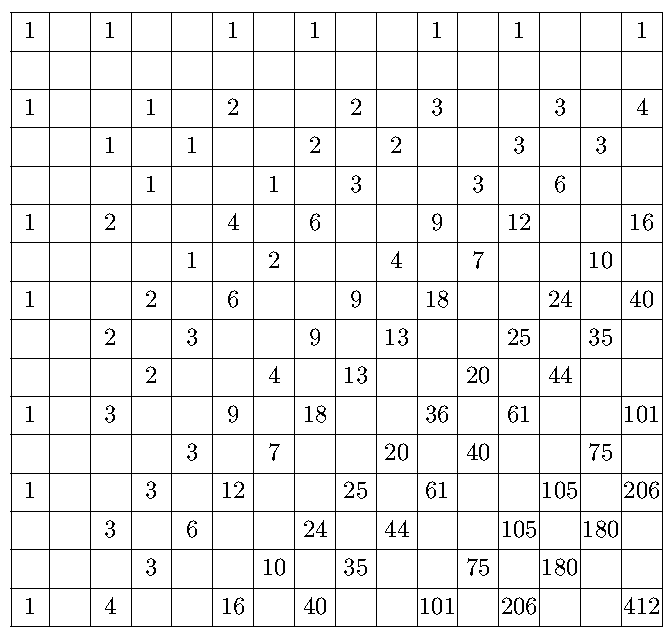
\includegraphics{obrazky/62D1}
\end{center}
Rovnako ako v~prvom riešení prichádzame k~výsledku 412.\\
\\
\begin{tcolorbox}[breakable,notitle,boxrule=0pt,colback=light-gray,colframe=light-gray]\ul{24.8} [61-I-6]
Na hracej ploche $n \times n$ tvorenej bielymi štvorcovými políčkami sa Monika a Tamara striedajú v~ťahoch jednou figúrkou pri nasledujúcej hre. Najskôr Monika položí figúrku na ľubovoľné políčko a toto políčko zafarbí namodro. Ďalej vždy hráčka, ktorá je na ťahu, urobí s~figúrkou skok na políčko, ktoré je doposiaľ biele, a toto políčko zafarbí namodro. Pritom pod skokom rozumieme bežný ťah šachovým jazdcom,  t.\,j. presun figúrky o~dve políčka zvislo alebo vodorovne a súčasne o~jedno políčko v~druhom smere. Hráčka, ktorá je na rade a už nemôže urobiť ťah, prehráva. Postupne pre $n = 4, 5, 6$ rozhodnite, ktorá z~hráčok môže hrať tak, že vyhrá nezávisle na ťahoch druhej hráčky.

\end{tcolorbox}

\rieh Ak je celkový počet políčok hracej plochy párny (v~zadaní pre $n = 4$ a $n = 6$), môže v~poradí druhá hráčka pomýšľať na túto víťaznú stratégiu: spárovať všetky políčka hracej dosky do dvojíc tak, aby v~každom páre boli políčka navzájom dosiahnuteľné jedným skokom. Pokiaľ také spárovanie políčok druhá hráčka nájde, má víťaznú stratégiu: v~každom ťahu urobí skok na druhé políčko toho páru, na ktorého prvom políčku figúrka práve leží.

Ak je celkový počet políčok hracej plochy nepárny (v~zadaní pre $n = 5$), môže v~poradí prvá hráčka pomýšľať na túto víťaznú stratégiu: spárovať všetky políčka hracej dosky okrem jedného do dvojíc tak, aby v~každom páre boli políčka navzájom dosiahnuteľné jedným skokom. Pokiaľ také spárovanie prvá hráčka nájde, má víťaznú stratégiu: v~prvom ťahu položí figúrku na (jediné) nespárované políčko a v~každom
ďalšom ťahu urobí skok na druhé políčko toho páru, na ktorého prvom políčku figúrka práve leží.

Nájsť požadované spárovania políčok je pre zadané príklady ľahké a je to možné urobiť viacerými spôsobmi. Ukážme tie z~nich, ktoré majú určité črty pravidelnosti. Na obr. 1 zľava je vidno, ako je možné spárovať políčka časti hracej plochy o~rozmeroch $4\times2$; celú hraciu plochu $4 \times 4$ rozdelíme na dva také bloky a urobíme spárovanie v~každom z~nich. I~na spárovanie políčok hracej plochy $6\times 6$ môžeme využiť spárovanie v~dvoch blokoch $4 \times 2$; na obr. 1 uprostred je znázornené možné stredovo súmerné spárovanie všetkých políčok. Nakoniec na obr. 1 vpravo je príklad spárovania políčok hracej plochy $5 \times 5$ s~nespárovaným políčkom v~ľavom hornom rohu (nespárované políčko nemusí byť nutne rohové); opäť je pritom využitý jeden blok $4 \times 2$.
\begin{center}
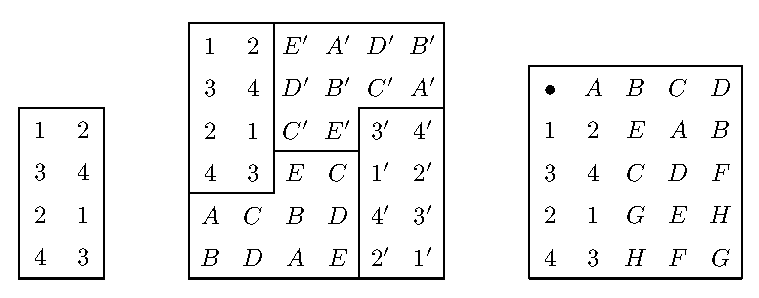
\includegraphics{obrazky/61D6} \\

Obr. 1
\end{center}
